\documentclass[11pt,english]{article}

\usepackage[english]{babel}
\usepackage{enumitem}
\usepackage{fancyhdr}
\usepackage{graphicx}
\usepackage{lastpage}

\pagestyle{fancy}

\graphicspath{{assets/}}

\lfoot{}
\cfoot{\today}
\rfoot{\thepage/\pageref{LastPage}}

\newcommand*{\Frontpage}{\begingroup
  \hbox{%
    \hspace*{0.2\textwidth}
    \rule{1pt}{\textheight}
    \hspace*{0.05\textwidth}
    \parbox[b]{0.75\textwidth}{%
      {\noindent\Huge\bfseries IDPRI}\\[2\baselineskip] % Title
      {\large \textit{Huiswerkopdrachten}}\\[4\baselineskip] % Tagline or further description
      {\Large \textsc{\\
          Patrick Spek, 2099745 \\
          Roy, 2097591 \\
        }}
      \vspace{0.5\textheight} % Whitespace between the title block and the publisher
    }
  }
\endgroup}

\renewcommand{\footrulewidth}{0.4pt}

\begin{document}
  \thispagestyle{empty}
  \Frontpage
  \newpage

  \tableofcontents
  \newpage

  \section{Mockups}
  \subsection{- scherm 1 -}
  \subsection{- scherm 2 -}

  \section{Stijl en kleur}
  \subsection{Stijl}
  Voor de stijl is gekozen voor een flat design. Dit ziet er moderner uit en is
  bekend bij praktisch iedereen die in de IT zit, zoals developers en managers
  die met bugs te maken hebben. Daarbij zijn flat icons goedkoper in
  bandbreedte, wat het zeer geschikt maakt voor mobile design. Hierdoor kunnen
  dezelfde icons gebruikt worden voor zowel de desktop als mobile applications.
  Hierdoor lijken de applicaties op elkaar, en hoeft de gebruiker niet opnieuw
  de icons te leren als ze van desktop naar mobile gaan.

  \subsection{Kleur}
  Voor de kleuren is gekozen voor een paars palette. De applicatie vraagt om
  creatieve geesten om bepaalde bugs op te lossen, dus het leek ons leuk om de
  applicatie ook een creatieve uitstraling te geven.

  \section{Mobile Wireframes}
  \subsection{Login}
  \makebox[\textwidth]{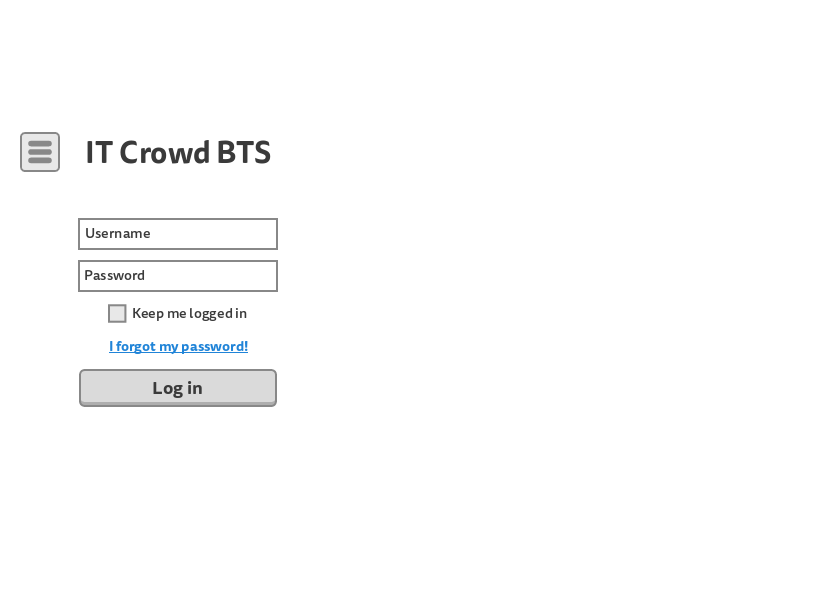
\includegraphics[width=\linewidth]{wfm-home}}

  \subsection{Dashboard}
  \makebox[\textwidth]{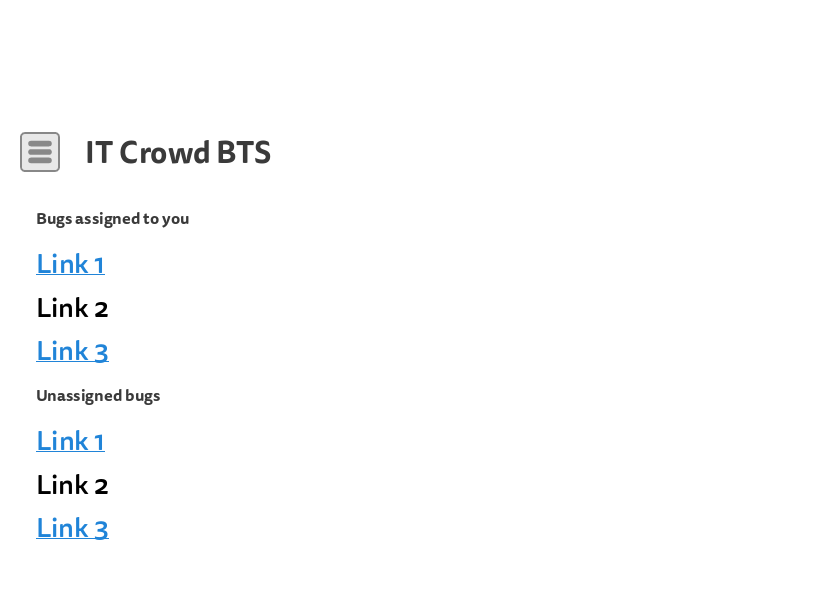
\includegraphics[width=\linewidth]{wfm-dashboard}}

  \subsection{Bug index}
  \makebox[\textwidth]{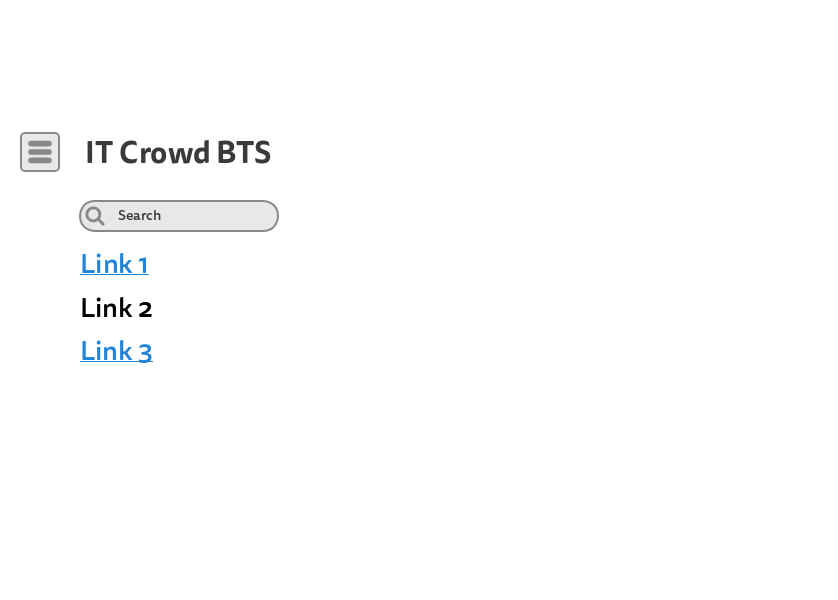
\includegraphics[width=\linewidth]{wfm-bugs}}

  \subsection{Bug view}
  \makebox[\textwidth]{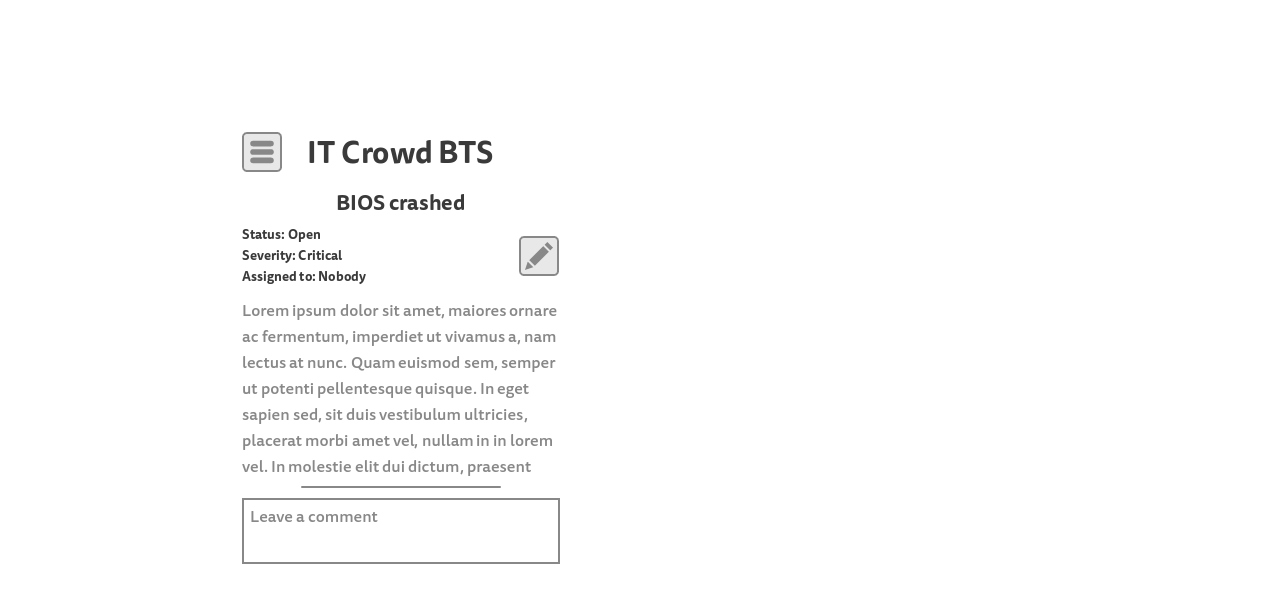
\includegraphics[width=\linewidth]{wfm-bug}}

  \subsection{Project index}
  \makebox[\textwidth]{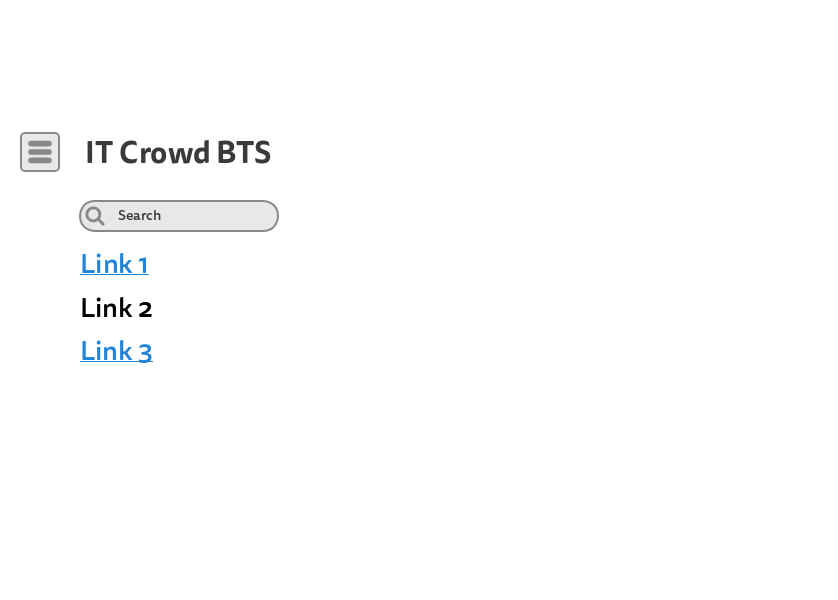
\includegraphics[width=\linewidth]{wfm-projects}}

  \subsection{Project view}
  \makebox[\textwidth]{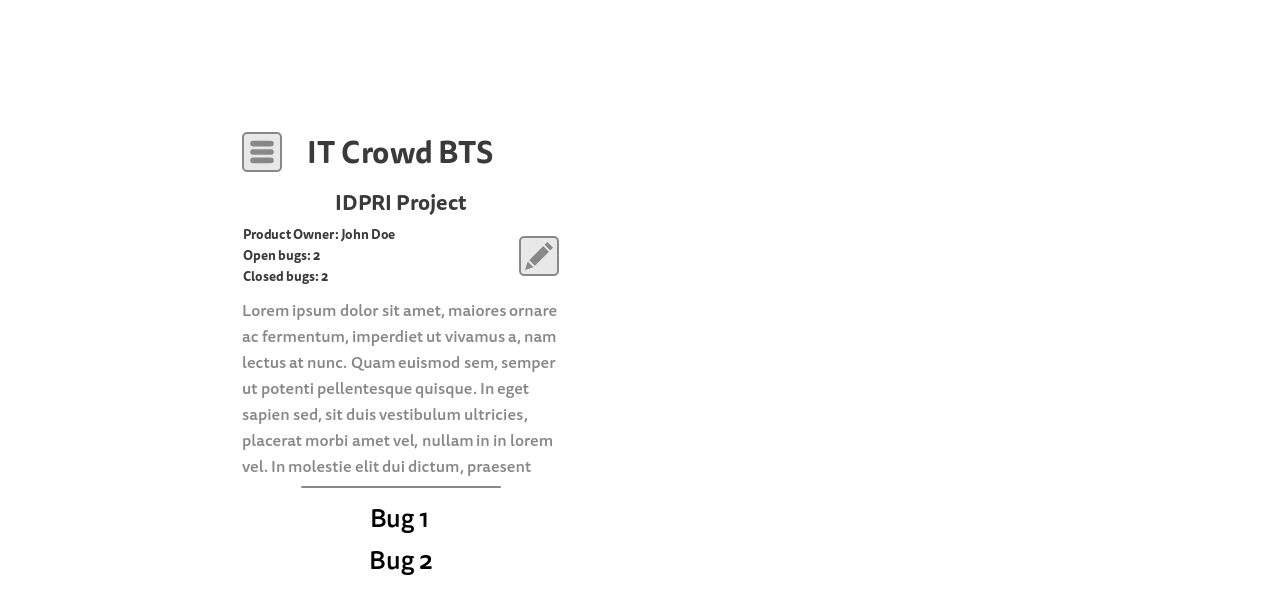
\includegraphics[width=\linewidth]{wfm-project}}

  \section{Mobile Design choices}
  We hebben gekozen om de lijsten kleiner te maken. Hierdoor is er misschien
  minder informatie beschikbaar in een oogopslag, maar er is genoeg informatie
  beschikbaar om snel even iets op te zoeken. Daarbij past het zo goed in het
  scherm en is er een zoekbalk toegevoegd om snel bij de juiste bug of project
  te kunnen komen.

  De assigned bugs zijn naar het beginscherm gegaan, zodat hier snel toegang
  tot is.

  Het menu aan de linkerkant is vervangen door een "hamburger" menu om ruimte
  te besparen, en in lijn te zijn met andere mobile applications. Dit maakt het
  voor de gebruiker makkelijker omdat deze al gewend is aan deze
  functionaliteiten.
\end{document}

